\documentclass{article}
\usepackage[utf8]{inputenc}
\usepackage{amsmath}
\usepackage{amsthm}
\usepackage{amssymb}
\usepackage{bm}
\usepackage{esdiff}
\usepackage{siunitx}
\usepackage[letter, portrait, margin=1in]{geometry}
\documentclass{article} 
\usepackage{hyperref}
\usepackage{enumitem}
\usepackage{fancyhdr}
\usepackage{fancybox}
\usepackage{lastpage} 
\usepackage{textgreek}
\usepackage{amsfonts}
\usepackage{extramarks}
\usepackage{physics}
\usepackage{amsthm}
\usepackage{bm}
\usepackage{graphicx}
\usepackage{xfrac}
\usepackage{minted}
\usepackage{xcolor} % to access the named colour LightGray
\definecolor{LightGray}{gray}{0.9}
\def\sr{{\mbox{$\resizebox{.09in}{.08in}{\includegraphics[trim= 1em 0 14em 0,clip]{ScriptR}}$}}}
\def\bsr{{\mbox{$\resizebox{.09in}{.08in}{\includegraphics[trim= 1em 0 14em 0,clip]{BoldR}}$}}}
\usepackage{amsmath}
\newcommand{\boxboi}[1]{\fbox {\parbox{\linewidth}{#1}}}

\title{CTA200 Assignment 3}
\author{Sam Lakerdas-Gayle}
\date{May 9, 2023}

\begin{document}

\maketitle

\newcommand{\pd}[2][]{\frac{\partial#1}{\partial#2}}

\section*{Question 1}
We define a point $c=x+iy$ on the complex plane with $-2<x<2$ and $-2<y<2$. Setting $z_0=0$ and iterating over the equation 
\begin{equation}
    z_{i+1}=z_i^2+c,
\end{equation}
results in either $z_i$ diverging to infinity, or stays small over large numbers of iterations (bound). The choice of $c$ alone decides whether $z_i$ is bound or diverges.

\vspace{0.3cm}
We use NumPy in Python to write a function that iterates over Equation 1 an arbitrary number of times, using a large number of different values of $c$. The function constructs the portion of the complex plane such that $-2<x<2$ and $-2<y<2$, and uses 2500 different values of $c$ to iterate over Equation 1. The function keeps track of which values of $c$ cause $z_i$ to diverge, and at which step of the iteration does $z_i$ diverge. We consider $z_i$ to diverge when $|z_i|>2$.

\vspace{0.3cm}
We use 200 iterations of Equation 1 for all points in the field. Figure 1 shows the values of $c$ that result in divergence in yellow and the values that are bound in black. Figure 2 shows, for each value of $c$, the iteration number that $z_i$ began to diverge. In other words, Figure 2 is coloured by $i$, where $i$ is the smallest value such that $|z_i|>2$. White values of $c$ did not diverge, while coloured values did converge.

\begin{figure}[h]
    \centering
    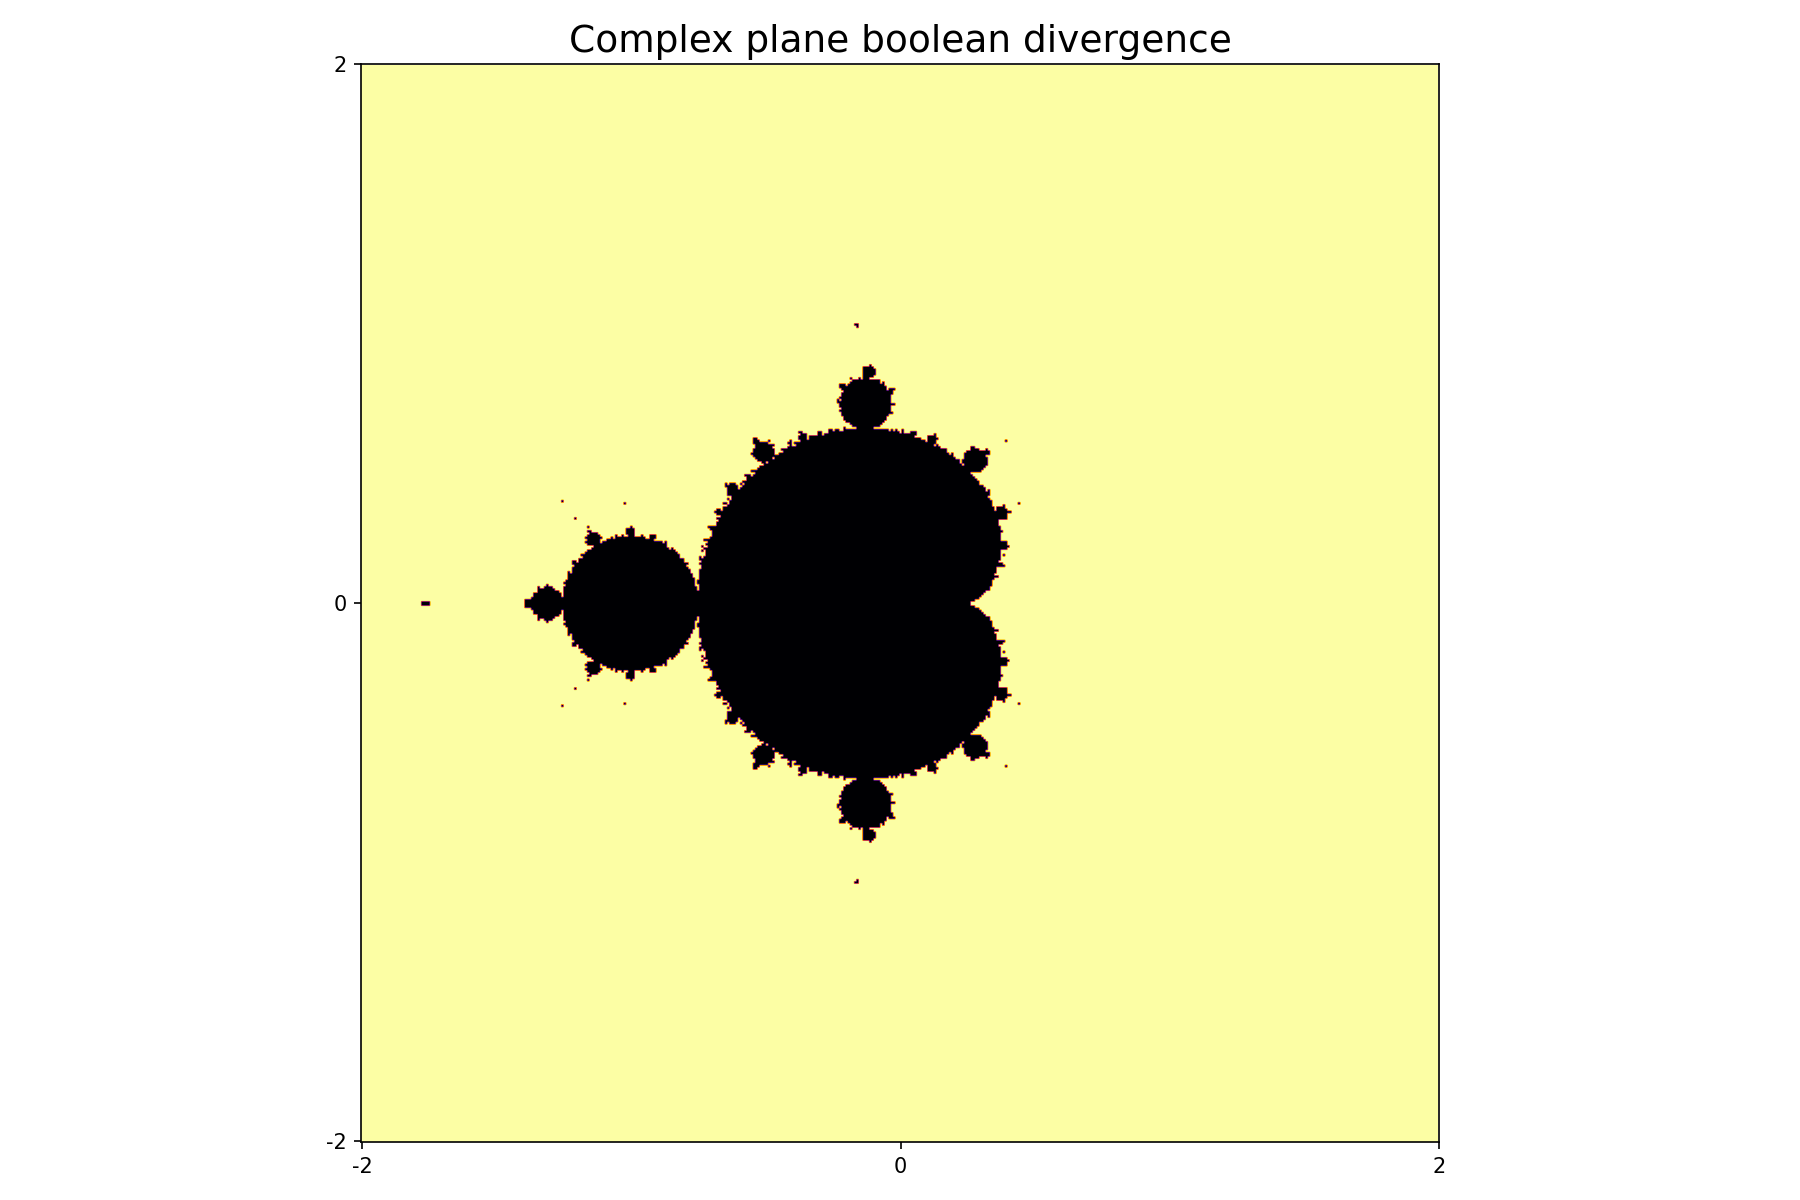
\includegraphics [scale=0.40]{Figures/bool_div.png}
    \caption{Values of $c$ in the complex plane, coloured yellow if $z_i$ diverges after 200 iterations of Equation 1, and coloured black if $z_i$ remains bound.}
    \label{fig:my_label4}
\end{figure}

\begin{figure}[h]
    \centering
    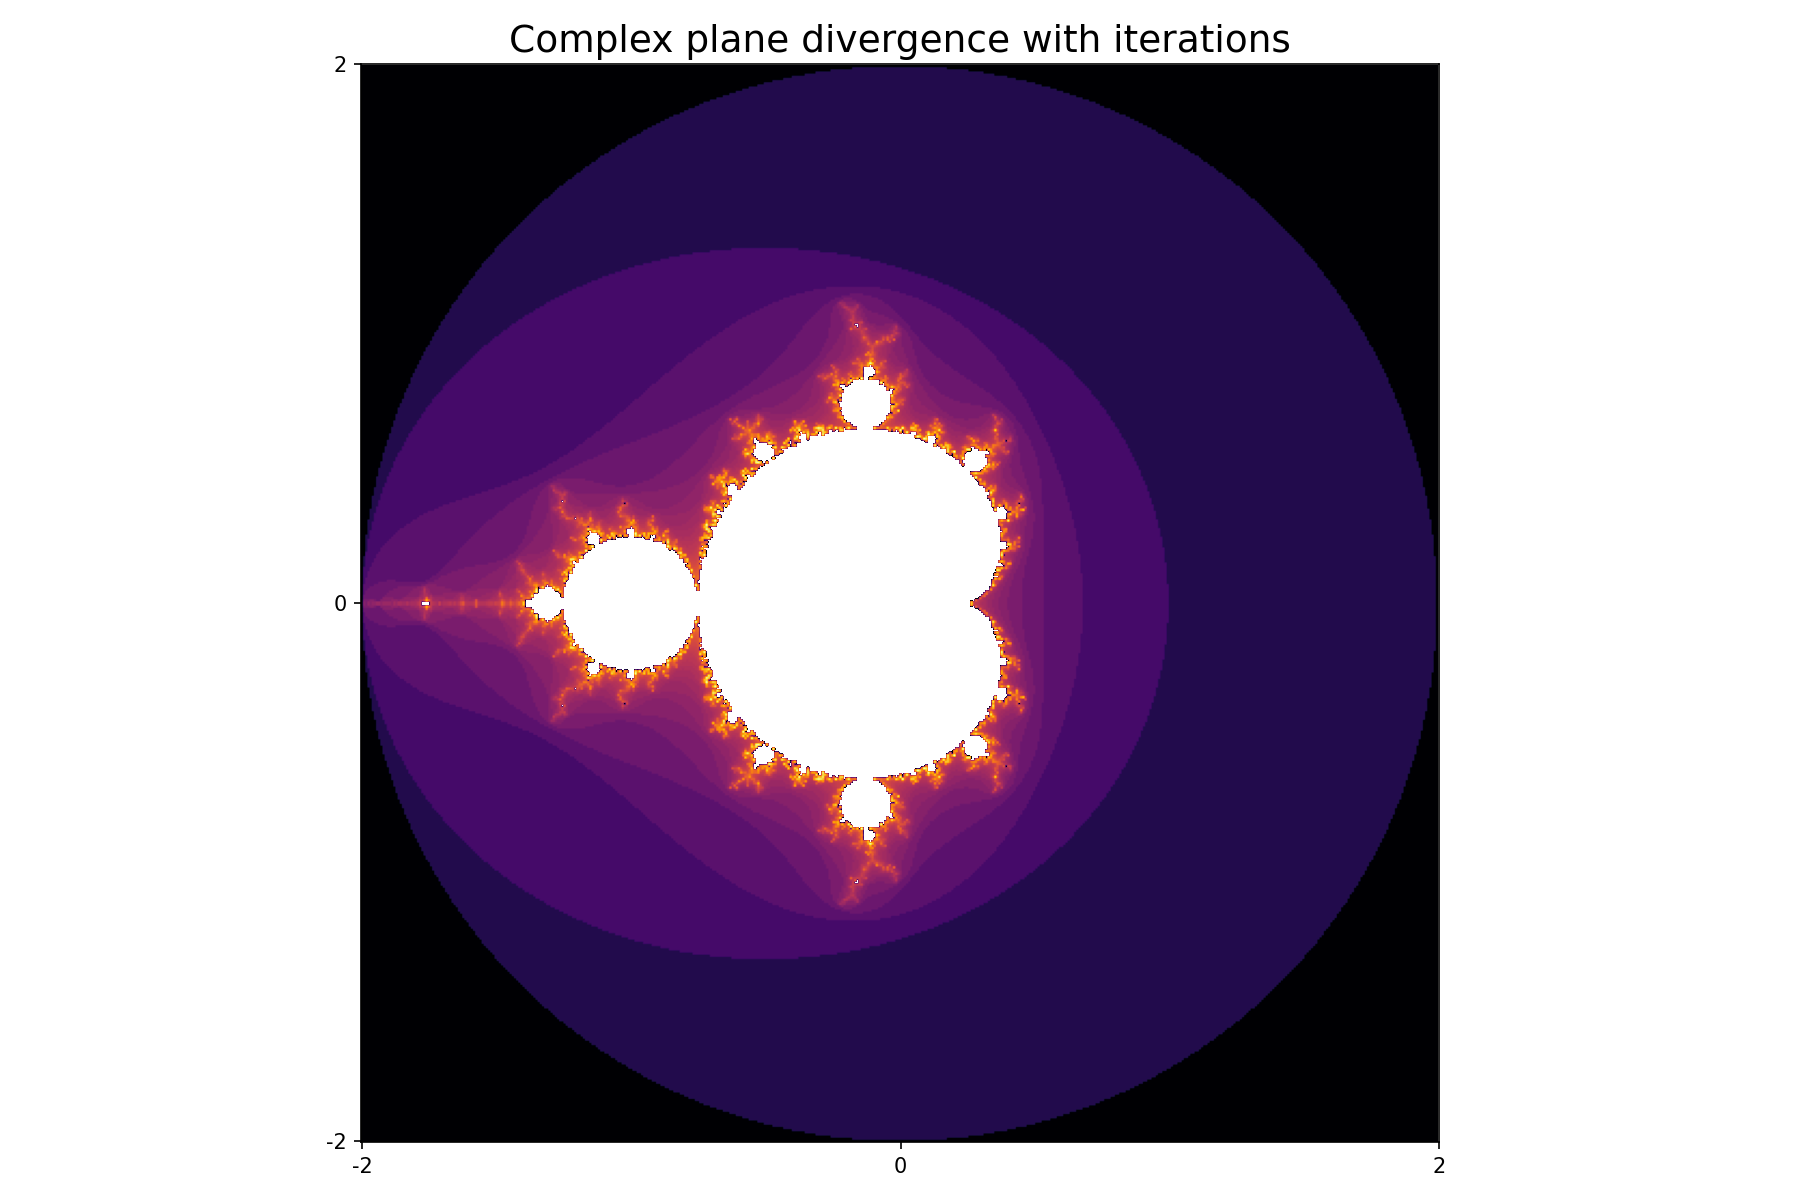
\includegraphics [scale=0.40]{Figures/itr_div.png}
    \caption{Values of $c$ in the complex plane, coloured based on the number of iterations of Equation 1 it takes for $z_i$ to diverge. Values range from 1 (darkest) to 200 (brightest). Values coloured in white result in bound $z_i$.}
    \label{fig:my_label4}
\end{figure}

\section*{Question 2}
Edward Lorenz's paper \href{https://journals.ametsoc.org/view/journals/atsc/20/2/1520-0469_1963_020_0130_dnf_2_0_co_2.xml}{Deterministic Nonperiodic Flow} outlines three ordinary differential equations
\begin{align}
    \dot{X}&=-\sigma(X-Y)\\
    \dot{Y}&=rX-Y-XZ\\
    \dot{Z}&=-bZ+XY,
\end{align}
where $W=(X,Y,Z)$ are three Fourier modes, $\sigma$ is the Prandtl number, $r$ is the Rayleigh number, and $b$ is a dimensionless length scale.

\vspace{0.3cm}
We solve Equations 2, 3, and 4 using SciPy's \textit{solve\_ivp} function. We use initial values of $W_0=(0, 1, 0)$, and we choose values of $\sigma=10, r=28, b=8/3$ as Lorenz does. We integrate over $t=60$ time units, with $100$ time steps per unit, so $6000$ total time steps. Solving for $X, Y,$ and $Z$ as a function of time, we obtain Figure 3, which closely aligns with Lorenz's figure.

\begin{figure}[h]
    \centering
    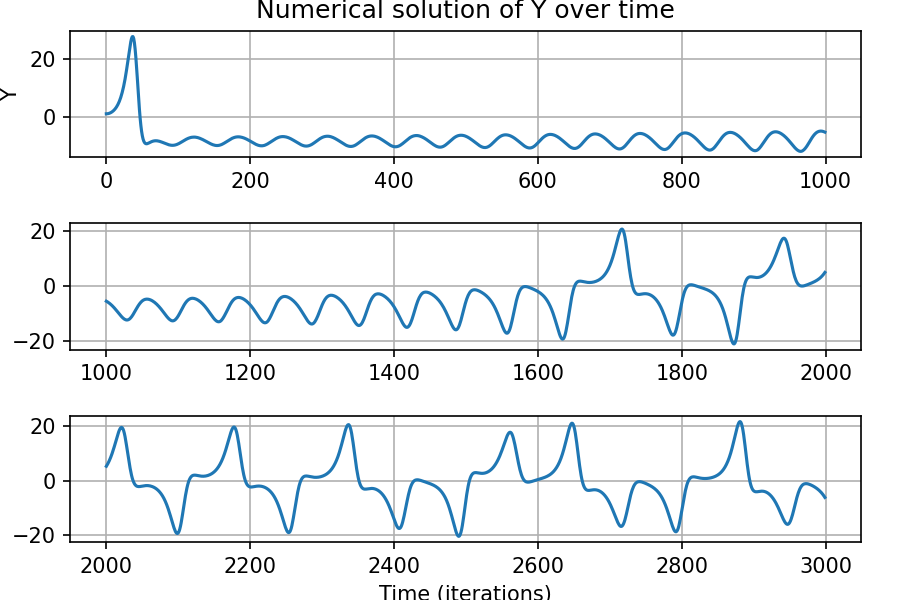
\includegraphics [scale=0.80]{Figures/num_sol.png}
    \caption{$Y$ as a function of time from $t=0$ to $t=30$. Each line represents 10 time units.}
    \label{fig:my_label4}
\end{figure}

\vspace{0.3cm}
Figures 4 and 5 show the solutions to $W$ in phase space, from $t=14$ to $t=19$. These plots are similar but not exactly what Lorenz obtained.

\begin{figure}[h]
    \centering
    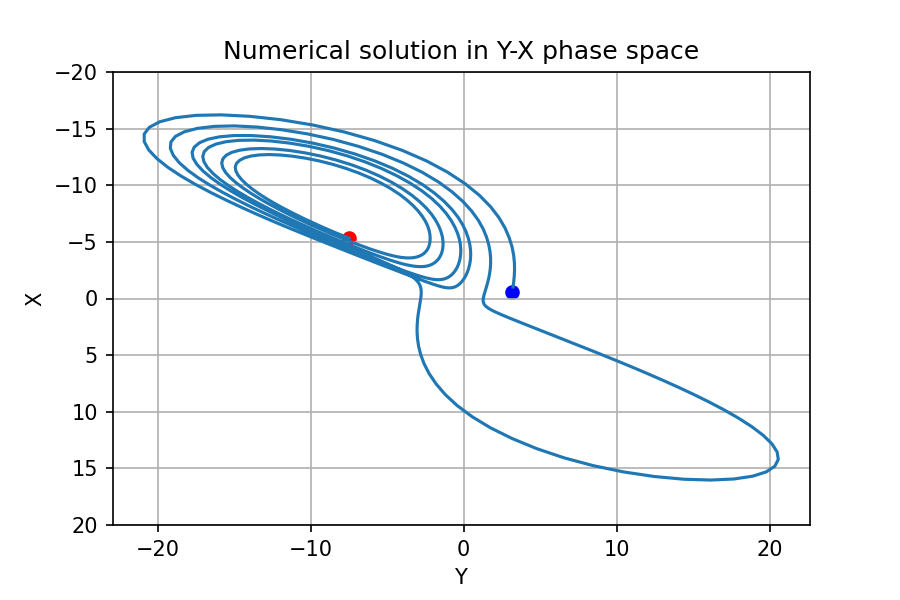
\includegraphics [scale=0.80]{Figures/yx_phase.png}
    \caption{Solutions to $X$ and $Y$ plotted in $Y-X$ phase space, from $t=14$ to $t=19$. The red dot is at $t=14$ and the blue dot is at $t=19$.}
    \label{fig:my_label4}
\end{figure}

\begin{figure}[h]
    \centering
    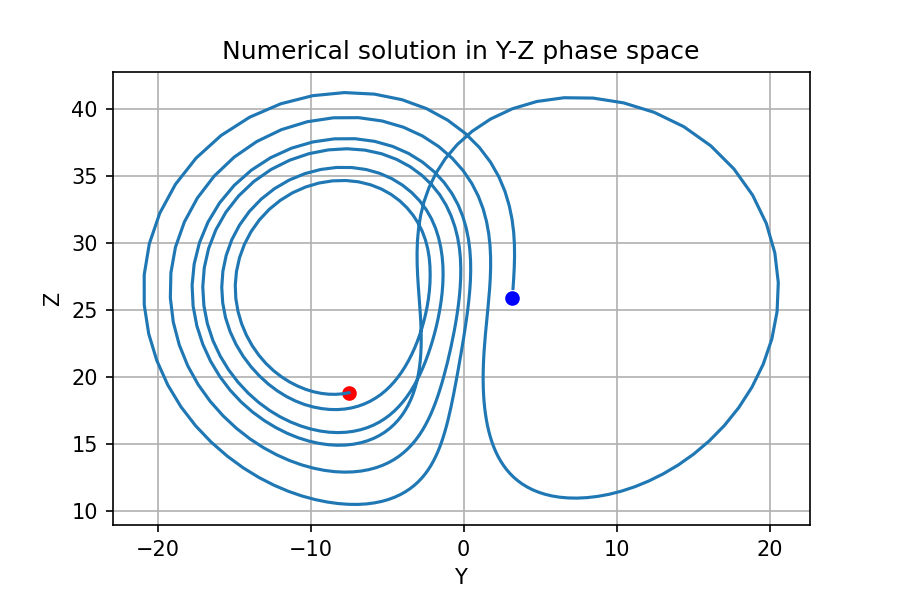
\includegraphics [scale=0.80]{Figures/yz_phase.png}
    \caption{Solutions to $Z$ and $Y$ plotted in $Y-Z$ phase space, from $t=14$ to $t=19$. The red dot is at $t=14$ and the blue dot is at $t=19$.}
    \label{fig:my_label4}
\end{figure}

\vspace{0.3cm}
We solve the initial value problem again, but this time we use the initial conditions $W_0'=W_0+(0,10^{-8},0)=(0, 1+10^{-8}, 0)$. After solving for $W'=(X', Y', Z')$ from using the initial condition $W_0'$, we calculate the distance between $W$ and $W'$, which we call the error, and plot the log of the error in Figure 6. We find that the log error is mostly linear in time, suggesting that a small fluctuation in the initial conditions cause exponential errors in the solutions.

\begin{figure}[h]
    \centering
    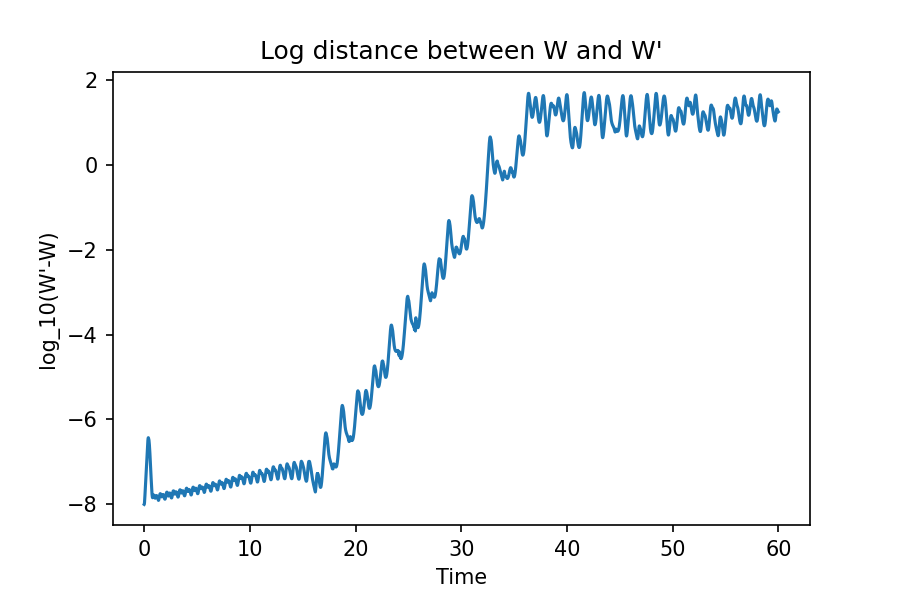
\includegraphics [scale=0.80]{Figures/err_w.png}
    \caption{Log error between W and W'. The log error is mostly linear in time, so the error is exponential.}
    \label{fig:my_label4}
\end{figure}

\vspace{0.3cm}
As seen from Figures 3, 4, and 5, the solutions to $W$ are close to Lorenz's solutions but are not exact. This is because we took a numerical method to solve the initial value problem. Different numerical methods may produce slightly different results, and the number of time steps will also affect the accuracy. As seen from Figure 6, this initial value problem is highly dependent on the prior conditions. So small errors in the numerical method turn into large errors in the solution.


\end{document}
